% !TeX spellcheck = en_US
\documentclass[french]{yLectureNote}

\title{Atomistique 2 - PS}
\subtitle{Chimie}
\author{Paulhenry Saux}
\date{\today}
\yLanguage{Français}

\professor{J.Cunny}
\usepackage{graphicx}%----pour mettre des images
\usepackage[utf8]{inputenc}%---encodage
\usepackage{geometry}%---pour modifier les tailles et mettre a4paper
%\usepackage{awesomebox}%---pour les boites d'exercices, de pbq et de croquis ---d\'esactiv\'e pour les TP de PC
\usepackage{tikz}%---pour deiffner + d\'ependance de chemfig
% \usepackage{tabularx}%---pour dimensionner automatiquement les tableaux avec variable X
\usepackage{awesomebox}%---Pour les boites info, danger et autres
\usepackage{menukeys}%---Pour deiffner les touches de Calculatrice
\usepackage{fancyhdr}%---pour les en-t\^ete personnalis\'ees
\usepackage{blindtext}%---pour les liens
\usepackage{hyperref}%---pour les liens (\`a mettre en dernier)
\usepackage{caption}%---pour la francisation de la l\'egende table vers Tableau
\usepackage{pifont}
\usepackage{array}%---pour les tableaux
\usepackage{lipsum}
\usepackage{yFlatTable}
\usepackage{multicol}
\newcommand{\Lim}[1]{\lim\limits_{\substack{#1}}\:}
\renewcommand{\vec}{\overrightarrow}
\newcommand{\N}[0]{\mathbb{N}}
\newcommand{\dd}{\mathrm{d}}
\newcommand{\norm}[1]{||\vec{#1}||}
\newcommand{\fo}{\psi(\vec{r},t)}
\newcommand{\foe}{\psi(\vec{r},t)\*}
\newcommand{\HH}{\hat{H}}
\newcommand{\hb}{\hbar}
\newcommand{\lap}{\nabla^2}
\newcommand{\lapcc}{\frac{\partial^2 }{\partial x^2}+\frac{\partial^2 }{\partial y^2}+\frac{\partial^2 }{\partial z^2}}
\begin{document}
\chapter{Rudiments de mécanique quantique}
\section{Les postulats de la mécanique quantique}
\subsection{Fonction d'onde}
\begin{theorem}[Postulat 1]
L'état d'un système à un instant t est complètement défini par la connaissance de sa fonction d'onde notée \(\fo\).
\end{theorem}
\begin{proposition}[Propriétés de la fonction d'onde]
Elle est normée (l'intégrale de sa différentielle vaut 1 sur tout l'espace). Elle n'a aucun sens physique mais \(|\fo|^2\) représente la densité de probabilité à la position et au temps donnés.
\end{proposition}
Ainsi :
\begin{itemize}
 \item \(\foe\fo\) est la probabilité de trouver la particule au point r.
 \item \(|\fo|^2\dd V\) est la probabilité de trouver la particule sur le volume infinitésimal dV
 \item \(\int_{0}^1\int_{0}^1\int_{0}^1 |\fo|^2\dd V\) est la probabilité de trouver la particule sur un cube de c\^oté 1.
 \item \(\int_{espace} |\fo|^2 \dd V = 1\)
\end{itemize}
\subsection{Opérateurs}
\subsubsection{Généralités}
\begin{theorem}[Opérateurs]
 À toute grandeur physique A mesurable on associe en mécanique quantique un opérateur linéaire et hermitique noté \^A. Ils prennent en entrée et sortie des fonctions d'onde.
\end{theorem}
\warningInfo{Scalaire}{Si l'opérateur \^A est simplement la multiplication par un scalaire \(\lambda\), on dit que \(\lambda\) est la valeur propre de \^A. \(\fo\) est alors le vecteur propre de \^A associé à la valeur propre \(\lambda\).}
\begin{definition}[Fonctions dégénérés]
Si 2 fonction différentes différentes donnent pour un m\^eme opérateur la m\^eme valeur propre, elles sont dites dégénérées.
\end{definition}
\begin{definition}[Fonctions propres]
Une fonction propre $\psi$ de \^A est une fonction non nulle telle que l'application de \^A sur $\psi$ donne \(k \psi\)
\end{definition}
\criticalInfo{Commutativité}{Les opérateurs ne commutent pas en général. 2 opérateurs commutent si \(\hat{A}\cdot \hat{B} - \hat{B}\cdot \hat{A} = 0\)}

\begin{myproof}[Une combinaison linéaire de fonctions propres dégénérées d'un opérateur est également fonction propre de cet opérateur avec la meme valeur propre]
Considérons une combinaison linéaire de ces fonctions propres dégénérées. Soit \(\theta\) une telle combinaison linéaire, \(\^A\) l'opérateur et \(k\) la valeur propre : \[\theta = c_1\psi_1+\dots+c_n\psi_n\]
Alors \begin{flalign*}
\hat{A} \theta &= \hat{A}(c_1\psi_1+\dots+c_n\psi_n)\\
&= \hat{A}c_1\psi_1+\dots+\^Ac_n\psi_n\\
&= kc_1\psi_1+\dots+kc_n\psi_n\\
&= k(c_1\psi_1+\dots+c_n\psi_n)\\
& = k\theta
\end{flalign*}
\end{myproof}
\begin{definition}[Opérateur hermitique]
Un opérateur hermétique donne des valeurs propres réelles et des vecteurs propres orthogonaux.
\end{definition}
\subsubsection{Principe de correspondance}
\begin{theorem}[Principe de correspondance]
 Tout opérateur peut \^etre construit à partir des opérateurs position et quantité de mouvement.
\end{theorem}
\begin{definition}[Opérateur position et quantité de mouvement]
Ils sont associés à une coordonnée (x,y,z). L'opérateur position consiste à multiplier par la coorodonnée et l'opérateur quantité de mouvement à dériver par rappot à la coordonnée puis à multiplier par \(-i \hbar\)
\end{definition}
Ainsi, \begin{itemize}
        \item \(\hat{q_i} = q_i \times\)
        \item \(\hat{p_x} = -i\hbar \frac{\partial}{\partial x}\)
        \item \(\hat{p} = -i\hbar \nabla\)
       \end{itemize}
\subsubsection{Opérateur Énergie et Hamiltonien}
\begin{definition}[Opérateur Énergie cinétique]
\[\hat{T} = - \frac{\hbar^2}{2m}\nabla^2\]
\end{definition}
\begin{definition}[Opérateur hamiltonien]
\[\hat{H} = \hat{T} + \hat{V}\] avec V l'énergie potentielle de la particule.
\end{definition}
\subsection{Équation de Schrodinger}
L'état d'un système est régie par \[\hat{H} \fo = i\hbar \frac{\partial \fo}{\partial t}\] Si le potentiel ne dépend pas du temps, le système est dans un état stationnaire (aussi appelé état propre du système\marginInfo{En effet, les fonctions d'onde sont alors les vecteurs propres associées à \(\^H\) car E est un scalaire}) et la fonction d'onde est obtenue par \[\hat{H}\fo = E\fo\] avec t constant.
\subsection{Mesure physique}
\begin{theorem}[Valeurs expérimentales]
 Les valeurs de A mesurables en peuvent \^etre que les valeurs propres de l'opérateur associé \(\^A\)
\end{theorem}
Si la fonction d'onde n'est pas une fonction propre de l'opérateur, alors la valeur moyenne des mesures sur la grandeur physique sera
\begin{proposition}[Valeur moyenne]
\refname{prop1}
\[<A> = \frac{\int\int\int \foe\^A\fo \dd V}{\int\int\int\foe \fo \dd V}\]
\end{proposition}

La dispersion sera alors \[\sqrt{<A^2>-<A>^2}\]
\section{Application des postulats}
\subsection{En 1D}

\includegraphics[scale=0.5]{figures/fig1}

On souhaite déterminer la fonction d'onde décrivant la particule dans la situation suivante : \(V_1 = \infty, V_0 = 0\). La particule ne peut se trouver que dans la zone du milieu\marginCheck{En effet, une zone avec un potentiel infini ne peut contenir la particule.} de l'axe \(x\). On va donc résoudre l'équation de Schrodinger pour cette zone.

Calculons d'abord l'hamiltonien :
\begin{flalign*}
\HH &= \hat{T} + \hat{V}\\
&= -\frac{\hb}{2m}\lap + \hat{0}\\
&= -\frac{\hb}{2m}(\lapcc)\\
&= - \frac{\hb}{2m}(\frac{\partial^2}{\partial x^2})
\end{flalign*}
Injectons le dans l'equation de Schrodinger :
\begin{flalign*}
- \frac{\hb}{2m}\frac{\partial^2}{\partial x^2} \psi(x) &= E \psi(x)\\
- \frac{\hb}{2m}\frac{\partial^2}{\partial x^2} \psi(x) -E \psi(x) &= 0\\
\frac{\partial^2}{\partial x^2} \psi(x) + \frac{2mE}{\hb}\psi(x) &= 0
\end{flalign*}
En posant \(k^2 = \frac{2mE}{\hb}\), on obtient l'équation différentielle :
\[\frac{\partial^2}{\partial x^2} \psi(x) + k^2 \psi(x) = 0\] que l'on sait résoudre.
Les solutions sont de la forme \(\psi(x) = A\cos(kx) + B\sin(kx)\). Pour déterminer A et B, on se sert des Propriétés des fonctions d'onde.

Les fonctions d'onde sont continues, donc \(\psi(0) = \psi(L) = 0\). On en déduit que \(A = 0\). Donc \[\psi(x) = B\sin(kx)\]
En évaluant la fonction en L, on obtient \(\psi(L) = B\sin(kL) = 0\). Comme B ne peut pas \^etre nul,\marginCheck{En effet, cela signifirait que la fonction est tout le temps nul, or c'est impossible car la particule existe bien.} c'est le sinus qui l'est. Cela nous amène à poser \(KL = \pi n\) avec \(n\in \mathbb{Z}\)\marginInfo{En mettant kL au carré, et en se servant de cette relation, on peut déduire une expression de l'énergie de la particule, c'est à dire la valeur propre de la fonction : \(E_n =\frac{\hb^2n^2\pi^2}{2mL^2}\). On remarque alors qu'on retrouve bien \(n\), ce qui montre que cette énergie est quantifiée et qu'elle ne peut prendre que certaines valeurs.}.

On a donc la forme générale de la fonction : \[\psi_n = B\sin(\frac{\pi n}{L}x)\] On va maintenant se servir de la condition de normalisation pour déterminer B.
\begin{flalign*}
\int_0^L |\psi_n(x)|^2 \dd x &= 1\\
|B|^2\int_0^L \sin^2(\frac{\pi n}{L}x)\dd x &= 1\\
|B|^2\int_0^L \frac{1-\cos(\frac{\pi n}{L}x)}{2} \dd x &= 1\\
\frac{|B|^2}{2}\int_0^L  \dd x - \frac{|B|^2}{2}\int_0^L \cos(\frac{\pi n}{L}x) \dd x &= 1\\
\frac{|B|^2}{2}\int_0^L  \dd x - 0 &= 1\\
\frac{|B|^2}{2}L &= 1\\
B &= \pm \sqrt{\frac{2}{L}}
\end{flalign*}

On va maintenant vérifier 2 propriétés
\subsubsection{Inégalité d'Heisenberg}
On souhaite vérifier \begin{theorem}[Inégalité d'Heinsenberg]
                      \(\Delta x\Delta p_x \geq \frac{\hb}{2}\)
                     \end{theorem}
Il faut donc calculer 4 termes :
\begin{itemize}
 \item \(<x> = \frac{2}{L}\int_0^L x \sin(\frac{\pi n}{L}x)\dd x = \frac{L}{2}\)
  \item \(<x^2> = \int_0^L \hat{x}^2 |\psi(x)|^2 \dd x\)
   \item \(<p_x> = \int_0^L \hat{p_x} |\psi(x)|^2 \dd x\)
  \item \(<p_x^2> = \int_0^L \hat{p_x}^2 |\psi(x)|^2 \dd x\)
\end{itemize}
On a utilisé la formule \ref{prop1} en remarquant que par la condition de normalisation, le denominateur vaut 1.
\subsubsection{Orthogonalité des vecteurs propres}
On veut vérifier que \[I = \int_0^L \psi_n^*(x)\psi_m^* \dd x = 0\]. On a donc
\begin{flalign*}
I &= \frac{2}{L} \int_0^L \sin(\frac{n\pi}{L}x)\sin(\frac{m\pi}{L}x) \dd x\\
&= \frac{1}{L} \int_0^L \cos(\frac{\pi}{L}(n-m)x)-\cos(\frac{\pi}{L}(n+m)x) \dd x\\
&= \frac{1}{L} \int_0^L \cos(\frac{\pi}{L}(n-m)x) \dd x - \frac{1}{L} \int_0^L \cos(\frac{\pi}{L}(n+m)x) \dd x\\
&= \frac{1}{L}\frac{L}{\pi(n-m)}[\sin(\frac{\pi}{L}(n-m)x)]_0^L-  \frac{1}{L}\frac{L}{\pi(n+m)}[\sin(\frac{\pi}{L}(n+m)x)]_0^L\\
&= 0
\end{flalign*}
On obtient bien 0 car les entiers \(m\) et \(n\) sont quelconques donc les sinus sont tous nuls.
\subsection{En 2D}
\subsubsection{Séparation des variables}
\begin{theorem}[Séparation des variables]
 Si on peut écrire un opérateur A comme la somme de 2 opérateurs s'appliquant à 2 variables, alors le produit des vecteurs propres des deux opérateurs et le vecteur propre de l'opérateur A. La somme des valeurs propres des 2 opérateurs vaut celle de A.
\end{theorem}
\subsubsection{Boite 2D}

\includegraphics[scale=0.5]{figures/fig2}

On calcule l'hamiltonien : \[\HH = -\frac{\hb^2}{2m}(\frac{\partial^2}{\partial x^2} + \frac{\partial^2}{\partial y^2}) = -\frac{\hb^2}{2m}(\frac{\partial^2}{\partial x^2}) -\frac{\hb^2}{2m}(\frac{\partial^2}{\partial y^2})\]
On voit que l'on peut séparer les variables en vertu du théorème précédent. On applique donc les résultats de la partie précédente. Ainsi,
\begin{itemize}
 \item \(\theta_{n_x}(x) = \pm \frac{2}{L_x}\sin(\frac{n_x\pi}{L_x}x)\)
  \item \(\theta_{n_y}(x) = \pm \frac{2}{L_y}\sin(\frac{n_y\pi}{L_y}y)\)
  \item \(E_{n_x} = \frac{\hb^2n_x^2\pi^2}{2mL_x^2}\)
  \item \(E_{n_y} = \frac{\hb^2n_y^2\pi^2}{2mL_y^2}\)
\end{itemize}
On en déduit, toujours par le théorème précédent que
\begin{itemize}
\item \(\psi_{n_xn_y}(x,y) = \pm \sqrt{\frac{2}{L_x}}\sqrt{\frac{2}{L_y}}\sin(\frac{n_x\pi}{L_x}x)\sin(\frac{n_y\pi}{L_y}y)\)
\item \(E_{n_x,n_y} = \frac{\hb^2\pi^2}{2m}(\frac{n_x^2}{L_x}+\frac{n_y^2}{L_y})\)
\end{itemize}
\subsection{Particule sur une sphère}
\subsubsection{Analyse}
\warningInfo{Rappel : condition de normalisation  en coordonnées sphériques}{Il faut que \[\int_0^{\infty}\int_0^{\pi}\int_0^{2\pi} \psi^*\psi r^2\sin(\theta)\dd \theta \dd \phi \dd r = 1\]}
On considère une particule de masse \(\mu\) évoluant à une distance r de l'origine. Il n'y a pas de potentiel ici, seul l'opérateur énergie cinétique est pris en compte :
\begin{flalign*}
\HH &= \frac{-\hb^2}{2\mu}\lap\\
&= \frac{-\hb^2}{2\mu} (\frac1{r^2}\frac\partial{\partial r}\left(r^2 \frac{\partial }{\partial r}\right) + \frac1{r^2 \sin \theta} \frac{\partial}{\partial \theta}\left(\sin \theta \frac{\partial}{\partial \theta}\right) + \frac1{r^2 \sin^2 \theta} \frac{\partial^2}{\partial \varphi^2})\\
&= \frac{-\hb^2}{2\mu} (\frac1{r^2 \sin \theta} \frac{\partial}{\partial \theta}\left(\sin \theta \frac{\partial}{\partial \theta}\right) + \frac1{r^2 \sin^2 \theta} \frac{\partial^2}{\partial \varphi^2})\\
&= \frac{-\hb^2}{2\mu}\hat{\wedge}
\end{flalign*}
Cela nous permet d'enlever une variable\marginCheck{En effet, r étant constant, sa dérivée est nulle} dans l'équation. On utilise ensuite le résultat suivant :
\begin{theorem}[Fonctions propres de l'opérateur de Legendre]
\[\hat{\wedge} Y_{lm}(\theta, \varphi) = -l(l+1)Y_{lm}(\theta, \varphi)\]
\end{theorem}
En multipliant par \(\frac{-\hb^2}{2\mu r^2}\), on obtient
\[H Y_{lm} = \frac{\hb^2}{2\mu r^2}l(l+1)Y_{lm}\]
\subsubsection{Vecteurs propres}
Les fonctions propres de \(\hat{\wedge}\) sont les harmoniques associées aux valeurs propres \(-l(l+1)\). Elles sont composées d'un scalaire garantissant la normalisation, d'une exponentielle complexe et d'un polynome de Legendre de degré \(l\). Elles sont sans dimension et définies au signe près.

Le nombre \(l\) (nombre quantique angulaire) prend les valeurs entières positives\marginCritical{Dans cette situation, il ne peut pas prendre la valeur nulle car cela signifirait une énergie nulle, ce qui est impossible} et \(m\) (nombre quantique magnétique) les valeurs entières entre \(-l\) et \(l\)\marginCritical{On en déduit que pour chaque valeur de l, il y a 2l+1 fonctions propres différentes.}.
\subsubsection{Moment cinétique}
Il y a une équivalence entre énergie cinétique en mécanique classique et quantique. En effet, on a
 \[E_c = \frac{L^2}{2\mu r^2}\]
 et \[E_q = \frac{\hb^2}{2\mu r^2}l(l+1)\]
On en éduit que la norme du moment cinétique dépend de l : \[L = \sqrt{l(l+1)}\hb\]. On peut aussi en déduire un nouvel opérateur :
\begin{definition}[Opérateur du moment cinétique en coordonnées sphériques]
\[\hat{L}^2 = -\hb^2\wedge\] et projeté sur z : \[\hat{L_z} = -i\hb \frac{\partial}{\partial \varphi}\]
\end{definition}
\section{Atomes hydrogénoïdes}
\begin{definition}[Atome Hydogénoide]
Il n'est constitué que d'un noyau et un électron
\end{definition}
\subsection{Équation de Schrodinger}
L'énergie du système est donnée par la somme des énergies cinétiques du noyau et de l'éectron ainsi que par le potentiel électron-noyau.

Les opérateurs associés sont :
\begin{itemize}
 \item \(\hat{T_e} = \frac{-\hb^2}{2m_e}\Delta_e\)
 \item \(\hat{T_N} = \frac{-\hb^2}{2m_N}\Delta_N\)
\item \(\hat{V_{eN}} = \frac{-1}{4\pi\epsilon_0}\frac{Z_e^2}{\hat{r}}\)
\end{itemize}
L'hamiltonien est donc \[\HH = \hat{T_e} + \hat{T_N}+\hat{V_{eN}}\] On remarque cependant que l'équation ne pourra \^etre résoulue car le rayon dépend de la position des 2 particules. Il faut donc simplifier l'équation.
\subsubsection{Problème à 2 corps}
En notant \(\mu\) la masse réduite et en se plaçant dans un repère centré\marginCheck{Cela permet à l'opérateur \(\hat{r}\) de dépendre uniquement des coordonnées de l'électron, ce qui rend l'équation solube par séparation des variables.} sur le noyau, on peut noter l'hamiltonien comme\marginCheck{Il décrit uniquement le mouvement relatif de l'électron par rapport au noyau.} \[\HH = \hat{T_{\mu}} + \hat{V_{eN}} = -\frac{\hb^2}{2\mu}\Delta \mu - \frac{1}{4\pi \epsilon_0}\frac{Z_e^2}{\hat{r}}\]
\subsubsection{Résolution}
Comme le potentiel autour du noyau présente une symétrie sphérique, on se place en coordonnées sphériques. Ainsi, en injectant l'expression de l'hamiltonien dans l'équation de Schrodinger, on obtient :
\[\HH \psi = (-\frac{\hb^2}{2m_er^2}(\frac{\partial}{\partial r}r^2\frac{\partial}{\partial r}+\wedge)-\frac{1}{4\pi \epsilon_0}\frac{Z_e^2}{r})\psi = E\psi\]

On peut montrer que l'opérateur \(\HH\) et \(\wedge\) commutent. On en déduit\marginInfo{On a vu que 2 opérateurs qui commutent admettent les m\^emes vecteurs propres. La valeur propre obtenu est une constante selon \(\theta, \varphi\) mais la fonction d'onde recherchée dépend aussi de r, on en déduit que \(\lambda = R(r)\) } que \[\psi(r, \theta, \varphi) = \lambda Y_{lm}(\theta, \varphi) = R(r)Y_{lm}(\theta, \varphi)\]

Comme on connait la forme de la partie angualaire, il nous reste à déterminer la partie radiale. On injecte pour cela la solution trouvée dans l'équation :
\begin{flalign*}
\HH \psi = (-\frac{\hb^2}{2m_er^2}(\frac{\partial}{\partial r}r^2\frac{\partial}{\partial r}+\wedge)-\frac{1}{4\pi \epsilon_0}\frac{Z_e^2}{r})\psi &= E\psi\\
(-\frac{\hb^2}{2m_er^2}(\frac{\partial}{\partial r}r^2\frac{\partial}{\partial r}R(r)Y_{lm}(\theta, \varphi)+\wedge R(r)Y_{lm}(\theta, \varphi))-\frac{1}{4\pi \epsilon_0}\frac{Z_e^2}{r})R(r)Y_{lm}(\theta, \varphi) &= ER(r)Y_{lm}(\theta, \varphi)\\
(-\frac{\hb^2}{2m_er^2}(Y_{lm}(\theta, \varphi)\frac{\partial}{\partial r}r^2\frac{\partial}{\partial r}R(r)+\wedge R(r)Y_{lm}(\theta, \varphi))-\frac{1}{4\pi \epsilon_0}\frac{Z_e^2}{r})R(r)Y_{lm}(\theta, \varphi) &= ER(r)Y_{lm}(\theta, \varphi)\\
(-\frac{\hb^2}{2m_er^2}(\frac{\partial}{\partial r}r^2\frac{\partial}{\partial r}R(r)+\wedge R(r))-\frac{1}{4\pi \epsilon_0}\frac{Z_e^2}{r})R(r) &= ER(r)\\
\end{flalign*}
On a ainsi trouvé la partie radiale de l'équation de Schrodinger\marginCheck{Pouvant se mettre sous la forme d'une équation de Laguerre, cette partie est solvable.}. On remarque que l'énergie n'est liée qu'à cette partie.
\subsection{Fonctions propres de l'équation radiale}
Notées \(R_{nl}(r)\), elles sont composées d'une constante de normalisation, d'un polyn\^ome et d'une exponentielle réelle décroissante. Elle dépend aussi de \(n\) et de \(l\). À la différence de la partie angulaire, \(l\) répond à la condition \(n>l\geq 0\)

Ces dernières sont normalisées :
Pour montrer que la partie radiale de l'orbitale atomique 1s est normalisée, nous devons vérifier que l'intégrale du carré de la fonction radiale, multipliée par $r^2$ (qui provient de l'élément de volume en coordonnées sphériques), sur tout l'espace est égale à 1.

La fonction radiale de l'orbitale 1s est donnée par :
\[ R_{1s}(r) = 2 \left(\frac{Z}{a_0}\right)^{3/2} e^{-\frac{Zr}{a_0}} \]
où :
\begin{itemize}
    \item $Z$ est le numéro atomique (pour l'hydrogène, $Z=1$)
    \item $a_0$ est le rayon de Bohr ($a_0 \approx 0.529 \times 10^{-10}$ m)
\end{itemize}

La condition de normalisation est :
\[ \int_0^\infty |R_{1s}(r)|^2 r^2 dr = 1 \]

Substituons l'expression de $R_{1s}(r)$ dans l'intégrale :
\begin{align*}
    &\int_0^\infty \left|2 \left(\frac{Z}{a_0}\right)^{3/2} e^{-\frac{Zr}{a_0}}\right|^2 r^2 \dd r \\
    &= \int_0^\infty 4 \left(\frac{Z}{a_0}\right)^3 \left(e^{-\frac{Zr}{a_0}}\right)^2 r^2 \dd r \\
    &= \int_0^\infty 4 \left(\frac{Z}{a_0}\right)^3 e^{-\frac{2Zr}{a_0}} r^2 \dd r\\
    &= 4 \left(\frac{Z}{a_0}\right)^3 \int_0^\infty r^2 e^{-\frac{2Zr}{a_0}} \dd r
\end{align*}

Pour évaluer cette intégrale, nous pouvons utiliser la formule générale de l'intégrale gamma, qui est :
\[ \int_0^\infty x^n e^{-ax} dx = \frac{n!}{a^{n+1}} \]

Dans notre cas, $x = r$, $n = 2$, et $a = \frac{2Z}{a_0}$.

Appliquons cette formule à notre intégrale :
\begin{align*}
    \int_0^\infty r^2 e^{-\frac{2Zr}{a_0}} \dd r &= \frac{2!}{\left(\frac{2Z}{a_0}\right)^{2+1}} \\
    &= \frac{2}{\left(\frac{2Z}{a_0}\right)^3} \\
    &= \frac{2}{\frac{8Z^3}{a_0^3}} \\
    &= \frac{2a_0^3}{8Z^3} \\
    &= \frac{a_0^3}{4Z^3}
\end{align*}

Maintenant, substituons ce résultat de l'intégrale dans l'expression complète de la normalisation :
\[ 4 \left(\frac{Z}{a_0}\right)^3 \left(\frac{a_0^3}{4Z^3}\right) \]

En simplifiant, nous obtenons :
\[ 4 \frac{Z^3}{a_0^3} \frac{a_0^3}{4Z^3} = 1 \]

Cependant, elles ne sont pas toutes orthogonales entre elles : En effet, il faut que la fonction d'onde le soit, donc il suffit que la partie radiale ou la partie angulaire soit orthogonale. Ainsi, la partie radiale est orthogonale uniquement si \(l\) est le même et \(n\) est différent.
\subsection{Formule de Rydberg}
L'énergie de l'éelctron ne dépend que de \(n\). En effet, pour un hydrogénoide, on a \[E_n = \frac{E_1(H)Z^2}{n^2}\]
On a également la formule de Rydberg\marginInfo{La constante \(R_H\) est une approximation car elle vient directmement de la résolution de l'équation radiale, que l'on a simplifier en supposant que le noyay était fixe. Or, ce n'est pas le cas, il y a donc un décalage} :

\begin{theorem}[Formule de Rydberg]
 La longueur d'onde émise par un changement d'énergie d'un électron est reliée avec le niveau d'énergie \(n\) : \[\frac{1}{\lambda}= \mathcal{R_H}Z^2(\frac{1}{n_a^2}-\frac{1}{n^2_d})\]
\end{theorem}
\criticalInfo{Séries à connaitre}{\begin{itemize}
\item Série de Lyman (ultraviolet) : Transition vers n=1
\item  Série de Balmer (visible) : Transition vers n=2
\item Série de Paschen (infrarouge) : Transition vers n=3
\end{itemize}
}
\begin{theorem}[Énergie d'un état excité pour un hydrogénoide]
 \[E_n = -\frac{13.6 Z^2}{n^2}\]
\end{theorem}

\subsection{À retenir}
\begin{itemize}
 \item Constante de Rydberg : 10967750 m\(^{-1}\)
 \item \(E_{H,1} = -13.6\) eV
\end{itemize}
\warningInfo{Nombres quantiques}{
\begin{itemize}
 \item \(n \in \mathbb{N}^+\) : nombre quantique principal
 \item \(l \in \mathbb{N}, \in [0, n-1]\) le nombre quantique angulaire
 \item \(m \in \mathbb{N}, \in [-l, l]\) le nombre quantique magnétique
\end{itemize}
}
\warningInfo{Moment cinétique}{
Un électron dans une OA(l,m) a un moment cinétique de \(L = \sqrt{l(l+1)\hb}\) et une composante selon z valant \(m\hb\)}
Toutes les OA correspondant une valeur de n donnée sont dans un m\^eme couche\marginWarning{Elles ont alors le m\^eme niveau d'énergie : elles sont dites dégénérées.}Celles qui ont en plus la m\^eme valeur de l sont dans la m\^eme valeur de l sont dans une sous-couche\marginWarning{m pouvant prendre 2l+1 valeurs différentes, il y a au maximum 2l+1 OA dans une sous-couche.}
\subsection{Partie angulaire}
Les expressions des harmoniques sphériques sont complexes pour \(m\neq 0\). On introduit donc les harmoniques sphériques réelles qui sont des combinaisons linéaires\marginCritical{On peut faire des combinaisons linéaires car toute combinaison linéaire de vecteurs propres dégénérés d'un opérateur (ici l'opérateur de Legendre, do'ù viennent les harmoniques sphériques) est vecteur propre de ce m\^eme opérateur, avec la m\^eme valeur propre} de ces harmoniques :\[S^{\pm}_{l|m|} = \frac{Y_{l,m}\pm Y_{l,-m}}{(^-i)\sqrt{2}} \] Ainsi, 2 fonctions complexes donnent 2 fonctions réelles\marginTips{Il n'y a pas d'apparition de fonctions car les fonctions complexes sont définies au signe près, donc il y a en fait 2 fonctions.}. En pratique, on somme les fonctions et on utilise les identités d'Euler pour transformer les exponentielles complexes en fonctions trigonométriques. La division par 2 provient de la condition de normalisation.
\subsubsection{Exemple pour l=1}
Exemple pour l=1 :

Les harmoniques sphériques complexes pour $l=1, m = \pm 1$ sont :
\begin{align*}
Y_1^0(\theta, \phi) &= \sqrt{\frac{3}{4\pi}} \cos\theta \\
Y_1^1(\theta, \phi) &= -\sqrt{\frac{3}{8\pi}} \sin\theta e^{i\phi} \\
Y_1^{-1}(\theta, \phi) &= \sqrt{\frac{3}{8\pi}} \sin\theta e^{-i\phi}
\end{align*}

L'harmonique $Y_{1,x}$ ($p_x$) est :

\begin{flalign*}
Y_{1,x}(\theta, \phi) &= \frac{1}{\sqrt{2}} \left( Y_1^{-1}(\theta, \phi) - Y_1^1(\theta, \phi) \right) \\
&= \frac{1}{\sqrt{2}} \left( \sqrt{\frac{3}{8\pi}} \sin\theta e^{-i\phi} - \left(-\sqrt{\frac{3}{8\pi}} \sin\theta e^{i\phi}\right) \right) \\
&= \frac{1}{\sqrt{2}} \sqrt{\frac{3}{8\pi}} \sin\theta (e^{-i\phi} + e^{i\phi}) \\
% En utilisant $e^{i\phi} + e^{-i\phi} = 2\cos\phi$ :
&= \frac{1}{\sqrt{2}} \sqrt{\frac{3}{8\pi}} \sin\theta (2\cos\phi) \\
&= \sqrt{\frac{3}{4\pi}} \sin\theta \cos\phi &
\end{flalign*}

L'harmonique $Y_{1,y}$ ($p_y$) est :
\begin{flalign*}
Y_{1,y}(\theta, \phi) &= \frac{i}{\sqrt{2}} \left( Y_1^{-1}(\theta, \phi) + Y_1^1(\theta, \phi) \right) \\
&= \frac{i}{\sqrt{2}} \left( \sqrt{\frac{3}{8\pi}} \sin\theta e^{-i\phi} + \left(-\sqrt{\frac{3}{8\pi}} \sin\theta e^{i\phi}\right) \right) \\
&= \frac{i}{\sqrt{2}} \sqrt{\frac{3}{8\pi}} \sin\theta (e^{-i\phi} - e^{i\phi}) \\
% En utilisant $e^{i\phi} - e^{-i\phi} = 2i\sin\phi$ :
&= \frac{i}{\sqrt{2}} \sqrt{\frac{3}{8\pi}} \sin\theta (-2i\sin\phi) \\
&= \sqrt{\frac{3}{4\pi}} \sin\theta \sin\phi &
\end{flalign*}
\subsection{Représentation}
\subsubsection{Parties angulaires}
On peut déterminer les invariances par rotation en analysant les fonctions trigonométriques présentes dans l'harmonique et en utilisant la correspondance entre coordonnées cartésiennes et sphériques. Par exemple, si la fonction présente \(\sin(\theta)\cos(\varphi)\), comme on sait que \(x = r \sin(\theta)\cos(\varphi)\), on en déduit qu'elle a une symétrie selon \(x/r\). Cela signifie que pour une valeur de \(x\) donnée, la fonction à la m\^eme valeur pour tout les points situés à une m\^eme distance r de l'origine\marginInfo{Il y a donc une symétrie de révolution autour de l'axe x}. On la note alors \(P_x\).

Ainsi, les harmoniques de type s sont sphériques, les p ont des lobes autour d'axes et les d ont 4 lobes ou 2 lobes et un anneau.
\criticalInfo{Surface nodale}{Il y a l surfaces nodales pour chaque fonctions.}
\subsubsection{Parties radiales}
\begin{theorem}[Points nodaux]
 Dans les fonctions radiales, il y a n-l-1 points nodaux. Les points nodaux en 0 ne sont pas comptés s'il y en a.
\end{theorem}
Pour les représenter, comme elles dépendent de 3 variables, il faut 4 dimensions, ce qui est impossible, on utilise donc des isosurfaces\marginTips{Elles relient les points où la fonction a une valeur constante.} de 2 couleurs pour identifier le signe.

À partir d'un schéma, on peut identifier l'OA en comptant le nombre de fois que le signe change depuis le centre ainsi qu'avec la forme puis en appliquant la formule précédente.
\subsection{Densité de probabilité de présence radiale}
La densité de probabilité de présence radiale est \[\rho_{nl}(r) = R^2_{nl}(r)r^2\]. C'est la seule fonction qui a un sens physique, contrairement à la fonction \(R_{nl}(r)\) seule. On remarque que l'extrema le plus grand de la fonction \(\rho\) est celui pour lequel r est le plus grand. Pour les déterminer, on dérive simplement \(\rho(r)\) et on prend le dernier maximum pour trouver la distance électron-noyau la plus probable.

Pour trouver la distance moyenne, on calcule l'intégrale\marginInfo{On peut retrouver cette expression en revenant à la définition de \(<r>\) donnée en première partie et à la définition de l'opérateur \(\hat{r}\).}
\begin{theorem}[Valeur moyenne de la partie radiale]
\[\int_0^\infty R^2_{nl}(r)r^3 \dd r\]
\end{theorem}
\subsubsection{Exemple : maximum de densité de probabilité de présence pour n=2, l=0}
La fonction radiale pour l'orbitale $2s$ est :
\begin{flalign*}
R_{2s}(r) &= \frac{1}{2\sqrt{2}} \left(\frac{Z}{a_0}\right)^{3/2} \left(2 - \frac{Zr}{a_0}\right) e^{-\frac{Zr}{2a_0}} &
\end{flalign*}

La densité de probabilité radiale est $P(r) = r^2 |R_{2s}(r)|^2$.
\begin{flalign*}
P(r) &= r^2 \frac{1}{8} \left(\frac{Z}{a_0}\right)^3 \left(2 - \frac{Zr}{a_0}\right)^2 e^{-\frac{Zr}{a_0}} &
\end{flalign*}

Posons une variable sans dimension $x = \frac{Zr}{a_0}$.
\begin{flalign*}
P(x) &= \frac{Z}{8a_0} x^2 (2-x)^2 e^{-x} &
\end{flalign*}

Pour trouver les extrema, nous dérivons $\ln(P(x))$ par rapport à $x$ et égalons à zéro\marginTips{C'est plus facile en appliquant le logaritme pour les produits de fonction} :
\begin{flalign*}
\frac{d(\ln P(x))}{dx} &= \frac{2}{x} - \frac{2}{2-x} - 1 = 0 \\
\frac{4 - 4x}{2x - x^2} &= 1 \\
x^2 - 6x + 4 &= 0 &
\end{flalign*}

Les solutions de cette équation du second degré sont :
\begin{flalign*}
x &= \frac{6 \pm \sqrt{(-6)^2 - 4(1)(4)}}{2} \\
&= \frac{6 \pm \sqrt{36 - 16}}{2} \\
&= \frac{6 \pm \sqrt{20}}{2} \\
&= 3 \pm \sqrt{5} &
\end{flalign*}

Les valeurs de $x$ correspondant aux extrema sont donc :
\begin{flalign*}
x_1 &= 3 - \sqrt{5} \quad (\approx 0.764) \\
x_2 &= 3 + \sqrt{5} \quad (\approx 5.236) &
\end{flalign*}

Convertis en rayons $r = \frac{a_0}{Z}x$ :
\begin{flalign*}
r_1 &= \frac{a_0}{Z} (3 - \sqrt{5}) \\
r_2 &= \frac{a_0}{Z} (3 + \sqrt{5}) &
\end{flalign*}
La distance de probabilité maximale est donc la valeur la plus grande, soit \[\frac{a_0}{Z} (3 + \sqrt{5})\]
\subsection{Spin}
\begin{definition}[Spin]
Propriété intrinsèque des particules, c'est un moment magnétique intrinsèque. On différencie le nombre quantique de spin \(s = 0.5\) et le nombre quantique magnétique de spin \(m_s = \pm 0.5\)
\end{definition}
\section{Annexe : représentation des OA angulaires}
On utilise la fonction $S$ générée dans le cas où la fonction originale est complexe.

\subsubsection{Pour l=0}
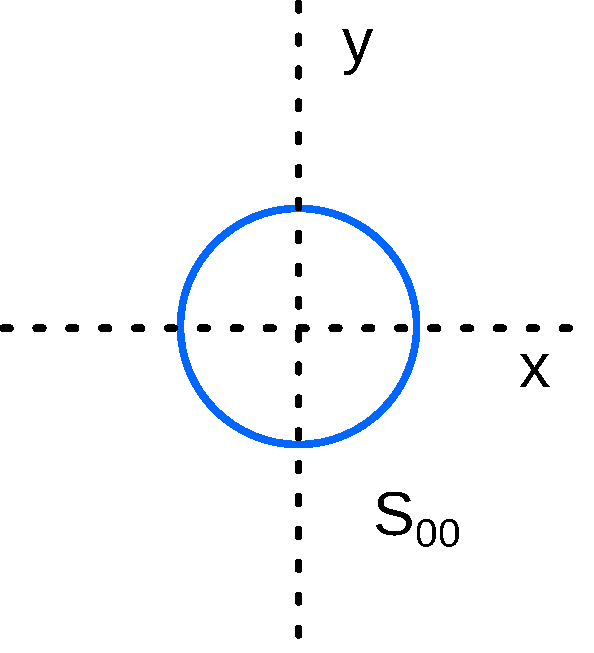
\includegraphics[scale=0.5]{figures/s00}
\subsubsection{Pour l=1}
On dit qu'elles ont une symétrie de révolution autour d'un certain axe
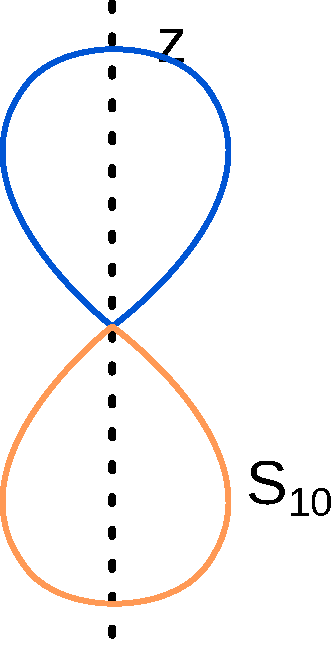
\includegraphics[scale=0.5]{figures/s10}
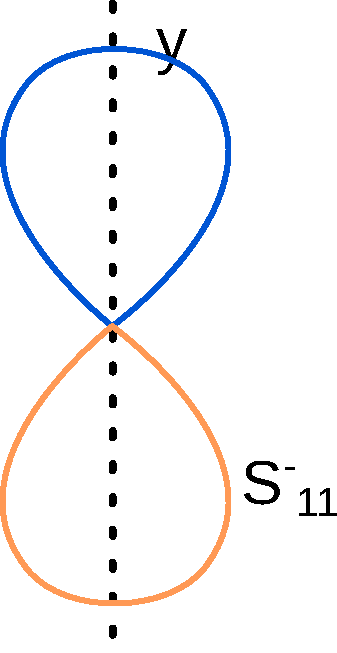
\includegraphics[scale=0.5]{figures/s-11}
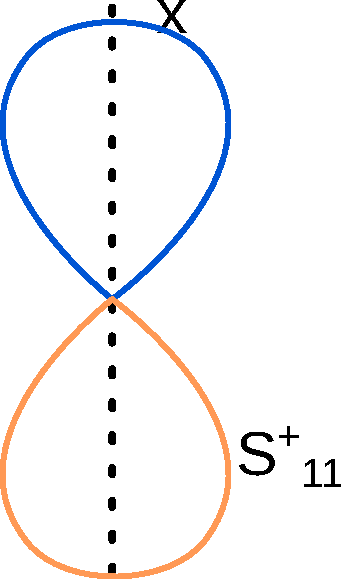
\includegraphics[scale=0.5]{figures/s+11}
\subsubsection{Pour l=2}
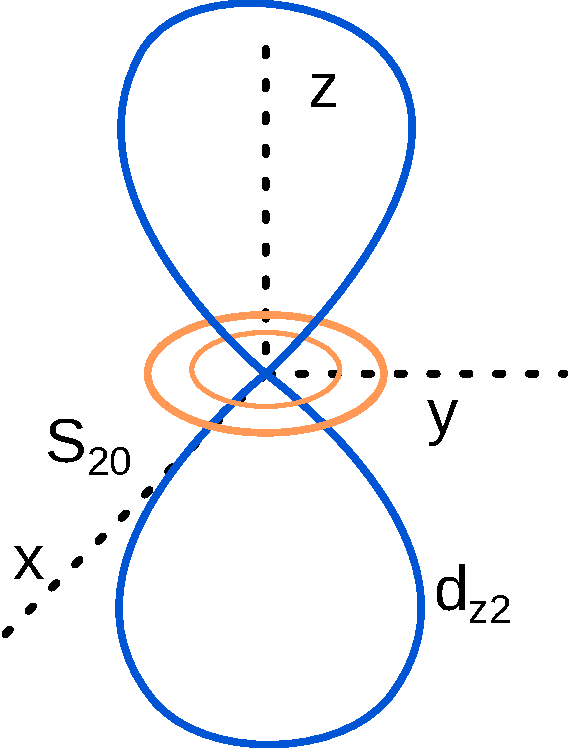
\includegraphics[scale=0.5]{figures/s20}
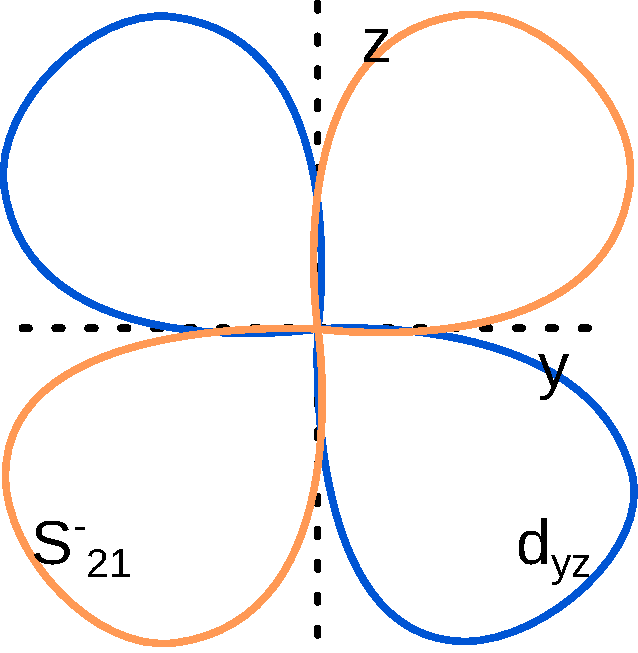
\includegraphics[scale=0.5]{figures/s-21}
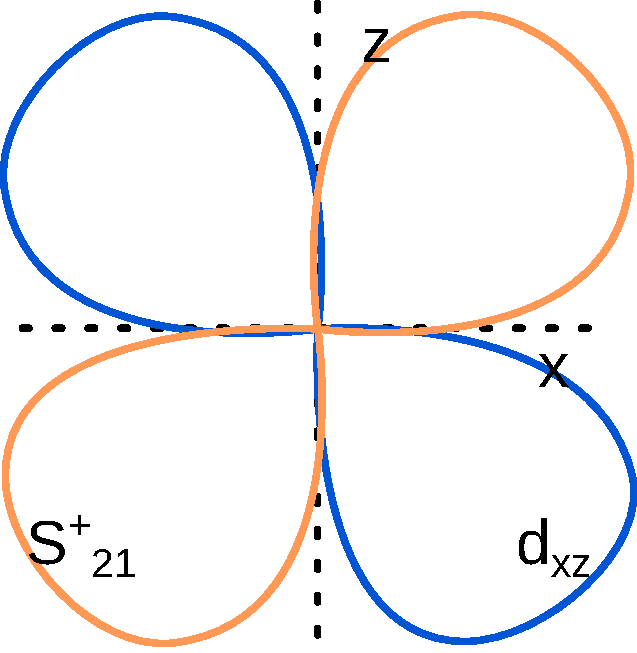
\includegraphics[scale=0.5]{figures/s+21}
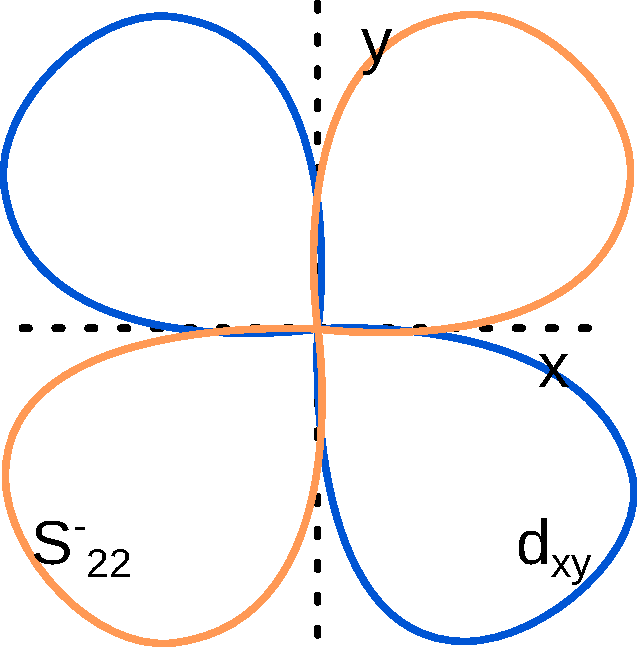
\includegraphics[scale=0.5]{figures/s-22}
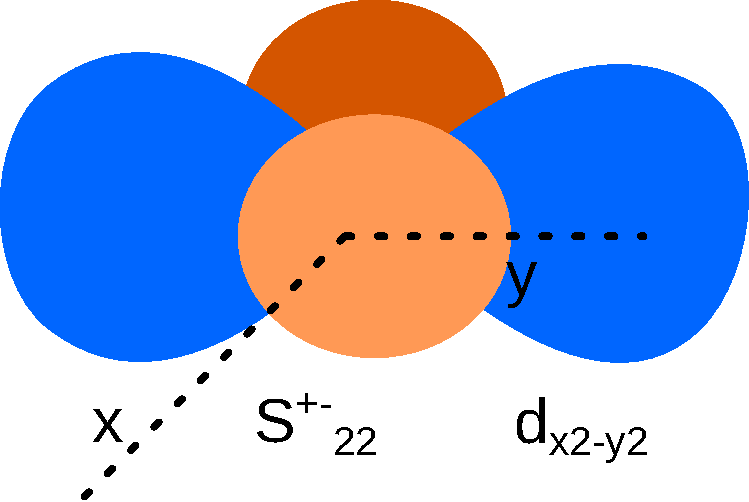
\includegraphics[scale=0.5]{figures/s+22}
 \end{document}
